\documentclass[a4paper]{article}
\RequirePackage[latin1]{inputenc}
\RequirePackage[T1]{fontenc}
\RequirePackage[ngerman]{babel}
\usepackage{graphicx}
\usepackage{a4wide}

\begin{document}
\begin{titlepage}
\author{Autor]}
\title{Implementierung eines einfachen Raytracers \\ ~ \\ ~ \\ 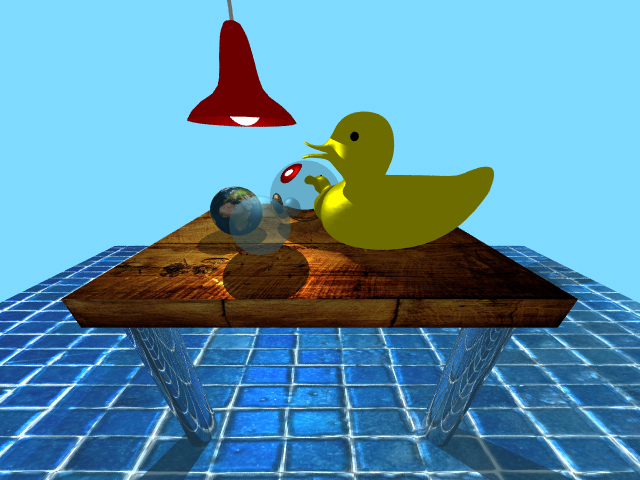
\includegraphics[width=\textwidth]{finish.png} \\ ~ \\ ~ \\ ~ \\ Praktikum WS 2011}
\author{Philipp Ruchti}
\end{titlepage}
\maketitle
\thispagestyle{empty}
\newpage
\setcounter{page}{1}
\section*{Raytracing}
Bei der gewohnten Erstellung eines Bildes, wie man es beispielsweise von OpenGL kennt werden die Vertices einer 3D-Szene mit Hilfe einer Projektionsmatrix auf eine Bildfläche projiziert und damit die Farbe eines Bildpunktes bestimmt. Beim Raytracing werden im Gegensatz hierzu Strahlen von der Kamera durch die Bildfläche geschickt und diese mit der 3D-Szene geschnitten. Diese Technik bietet die Möglichkeit auch Reflektionen, Schatten und viele andere Lichteffekte darzustellen. Im Gegensatz zur ersten Technik bietet Raytracing die Möglichkeit realistischere Bilder einer 3D-Szene zu berechnen ist jedoch rechenaufwendiger.
Im Verlaufe dieses Praktikums wurde ein einfacher Raytracer implementiert, welcher die grundlegenden Funktionalitäten bietet eine 3D-Szene abzubilden. Im folgenden werden die dafür verwendeten Techniken kurz erläutert.

\section*{Homogene Notation}
Um 3D-Positionen und Verschiebungen zu repräsentieren eignet sich die sogenannte homogene Notation. Hierzu werden 3D-Vektoren um eine vierte Komponente erweitert. Somit ist es auch mit Hilfe von 4x4-Matrizen möglich Punkte zu verschieben und zu rotieren und Vektoren zu rotieren. Punkte haben als 4.Komponente einen Wert $\neq 0$ welcher die die Länge des Vektors verändert. Vektoren welche eine 4. Komponente $= 0$ enthalten sind Richtungen, welchen eine unendliche Länge aufweisen und sich nicht verschieben lassen. Eine Matrix die einen Punkt mit einer Rotationsmatrix $\mathbf{M}$ rotiert und um $(x,y,z)$ verschiebt sieht homogen wie folgt aus:\\
\[\mathbf{M} = \left(\begin{array}{c}
\begin{array}{cr}
   \qquad \mathbf{R} ~~ & \begin{array}{c}
				x\\
				y\\
				z\\
			\end{array}\\
	\end{array}\\
	\begin{array}{cccc}
		0 & 0 & 0	& 1 \\
	\end{array}
	\end{array}
	\right)\]	 

\section*{Platzierung von Objekten und der Kamera}
Um Objekte und Kamera platzieren und verschieben zu können verwendet man homognene Matrizen. Hierbei erhält man das gleiche Ergebnis wenn man die Kamera in einer Richtung bewegt, oder alle Objekte in die entgegengesetzte Richtung bewegt, da für die Sicht in die Szene lediglich die relative Position von Kamera und Objekten eine Rolle spielt.
Um die Verwendung von AABBs zu vereinfachen wurde in dieser Implementierung die Kamera verschoben, beziehungsweise wurden die Strahlen nach Berechnung aus dem Ursprung und in kanonische Richtung mit Hilfe einer Transformationsmatrix verschoben und rotiert.

\section*{Strahlen - Objekt Schnittpunkt}
\subsection*{Implizite Oberflächen: hier Kugeln und Zylinder}
Implizite Oberflächen werden durch mathematische Gleichungen $f(x,y,z)$ beschrieben, welche für alle Punkt die auf der Oberfläche liegen $= 0$ ergeben. Für Kugeln benötigt man hierzu lediglich den Mittelpunkt der Kugel, sowie einen Radius. Die Punkte $(x,y,z)$ welche die Gleichung
\[f(x,y,z) = (x-u)^2 + (v-v)^2 + (z-w)^2 - r = 0\]
erfüllen bilden die Oberfläche einer Kugel mit Radius $r$ und Position $(u,v,w)$.

\subsection*{Parametrische Oberflächen: hier Drei- und Vierecke}
Parametrische Oberflächen sind Oberflächen welche durch eine Funktion $f(x,y)$ repräsentiert werden. Um die Kollision mit einer solchen Oberfläche zu berechnen muss man ein lineares Gleichungssystem lösen. Für Dreiecke bilden die Punkte welche die Gleichung
\[o+t\cdot d = (1 - b_1 - b_2)p_0 + b_1*p_1 + b_2*p_2\]
unter der Bedingung $b_1 \geq 0$ und $b_2 \geq 0$ und $b_1 + b_2 \leq 1$ erfüllen die Oberfläche. Für Vierecke ändert sich lediglich der letzte Teil der Bedingung zu $b_1 < 0$ und $b_2 < 0$.

\subsection*{AABBs}
Zur Beschleunigung der Schnittpunktberechnung kann um komplexere Objekte ein Boundingvolume gelegt werden. Die Kollisionsberechung mit diesem ist hierbei einfach und schnell zu berechnen und so müssen Strahlen, die das Boundingvolume nicht treffen nicht mit jedem Objekt des Inhaltes getestet werden. In der hier vorliegenden Implementierung wurden Axis-Aligned-Boundingboxes verwendet.

\section*{Phong Shading und Phong Beleuchtungsmodell}
Trift ein Strahl ein Objekt so wird an diesem zur Berechnung der "`gesehenen"' Objektfarbe sowohl die Farbe des Objektes beachtet als auch die Beleuchtung mit Hilfe der verschiedenen Lichtquellen berechnet, dies übernimmt das Beleuchtungsmodell. Für die Berechnung des hier verwendeten Beleuchtungsmodells wird ebenfalls die Normale des Punktes benötigt, dieses wird beim Phong Beleuchtungsmodell über das Objekt interpoliert. Die Beleuchtung an einer Stelle wird nach folgenden Formel berechnet:\\
\\$\mbox{Farbe} = \mbox{Farbe}_{ambient} \otimes E_{ambient} + \mbox{Farbe}_{diffuse} \otimes E_{diffuse} \cdot (n \cdot l) + \mbox{Farbe}_{specular} \otimes E_{specular} \cdot (R \cdot v)^m$\\\\
Hierbei ist $n$ die Normale am Objekt, $l$ die Richtung in welcher die Lichtquelle liegt $R$ die Refelktionsrichtung sowie $v$ die Sichtrichtung auf das Objekt.

\subsection*{Schatten}
\subsection*{Punktlichtquellen und gerichtete Beleuchtung}
Erweitert man obiges Modell um eine Prüfung ob die entsprechenden Lichtquellen gesehen werden, so kann man leicht Schatten erzeugen. Hierzu wird bei einer Punktlichtquelle ein Strahl von Punkt des Objektes, dessen Farbe soeben bestimmt wird, zur Lichtquelle geschickt und überprüft ob dieser auf dem Weg zum Licht ein Objekt trifft, ist dies der Fall so wird das Licht nicht gesehen. Handelt es sich um eine gerichtete Beleuchtung so darf kein Objekt in diese Richtung liegen, egal in welchem positivem Abstand.

\section*{Sampling}
Durch wenige Strahlen die durch die Bildpixel gesendet werden kann es bei kleinen Objekten oder feinen Strukturen dazu kommen, dass diese nicht oder Falsch dargestellt werden. Diesen Effekt kann man dadurch umgehen, dass man mehr Strahlen durch ein Bildpixel sendet und aus diesen danach einen Farbwert rekonstruiert. Um den Effekt des Aliasings zu reduzieren ist es zudem ratsam die Strahlen nicht geordnet anzulegen. Für diesen hier erstellten Raytracer wurden verschiedene Samplingmethoden zum Vergleich implementiert.

\subsection*{Random Sampling}
Beim Random Sampling werden durch ein Pixel mehrere Strahlen gesendet, die Position dieser ist hierbei zufällig und kann so dazu führen, dass eine unregelmäßige Deckung verschiedener Bereiche des Pixels erfolgt.

\subsection*{Stratified Sampling}
Beim Stratified Sampling wird das Pixel in mehrere regelmäßige \textit{Strata} eingeteilt, in jedem dieser Subregienen wird nun zufällig eine Position für einen Strahl ermittelt. Im Gegensatz zum Random Sampling verbessert sich die Deckung der verschiedenen Teilregionen des Pixels.

\subsection*{Poisson Sampling}
Für den hier implementierten Raytracer wurde das Verfahren des Poisson Sampling gewählt. Hierbei werden zufällig über das Pixel verteilt Orte gewählt, durch welche Strahlen gesandt werden sollen. Jedoch werden nur solche Positionen verwendet, die zu ihren Nachbarn einen gewissen Abstand aufweisen. So wird die Häufung der Strahlen an einer Stelle vermieden.

\subsection*{Halton Sampling}
Das ausgeklügeltste Sampling-Verfahren welches hier implementiert wurde ist das sogenannte Halton Sampling. Bei diesem Verfahren wird die Missverteilung des Positionen für die Strahlen minimiert. Hierzu werden sowohl die X- als auch die Y-Komponente der Position des Strahles anhand einer Hammerlesy Sequenz gewählt. Eine Hammerlesy Sequenz liefert Werte welche zwischen 0 und 1 liegen und diesen Bereich zu jedem Zeitpunkt möglichst gleich-verteilt abgedeckt.

\subsection*{Ergebnise der verschiedenen Sampling Methoden}
\begin{center}
	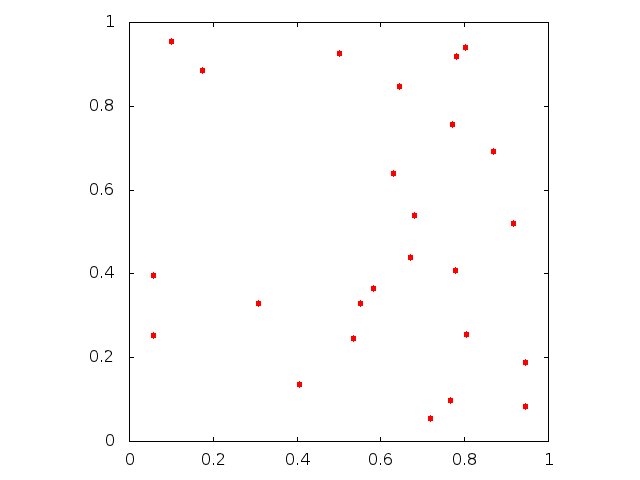
\includegraphics[width=0.45\textwidth]{random.png}~~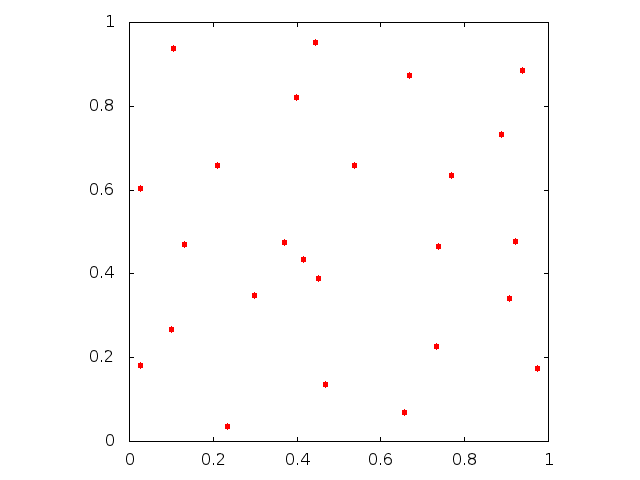
\includegraphics[width=0.45\textwidth]{stratified.png}\\
	\vspace{5pt}
	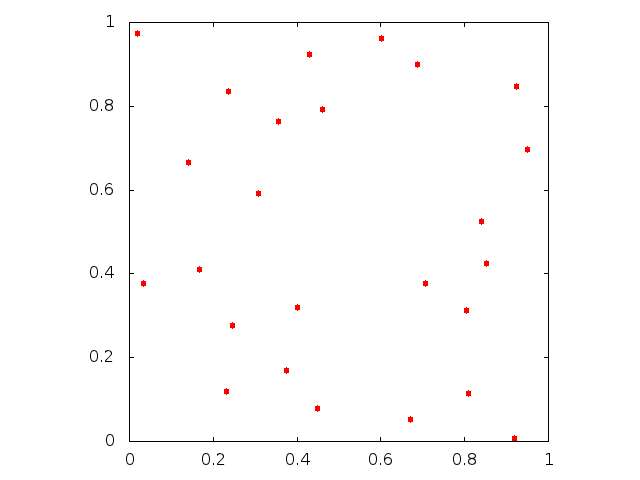
\includegraphics[width=0.45\textwidth]{poisson.png}~~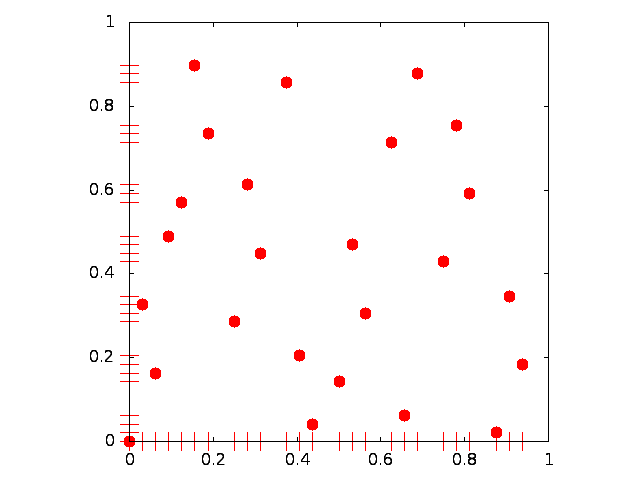
\includegraphics[width=0.45\textwidth]{halton.png}\\
\end{center}
Die von den verschieden Verfahren berechneten Positionen für Strahlen innerhalb eines Pixels. Von oben links nach unten rechts: Random Sampling, Stratified Sampling, Poisson Sampling, Halton Sampling (mit $p_1 = 2, p_2 = 7$).

\section*{Rekonstruktion}
Um aus den Farbwerten, welche die verschiedenen Strahlen die für den Bereich eines Pixels berechnen einen konsistenten Farbwert zu wählen bedarf es einer Rekonstruktionstechnik. Diese gewichtet die Farbwerte anhand eines Kernels $f(x,y)$ und normalisieret am Schluss das Ergebnis.

\subsection*{Box Rekonstruktion}
Ein einfaches Rekonstruktionsverfahren ist die Box-Rekonstruktion. Hierbei werden alle Farbwerte gleich gewichtet ($f(x,y) = 1$) und durch die Anzahl der Farbwerte geteilt, es wird also ein Mittelwert über alle vorhandenen Farbwerte der Strahlen gebildet.

\subsection*{Mitchell Rekonstruktion}
Die Mitchell Rekonstruktion gewichtet die Farbwerte mit einer Standart-Normalverteilung ihres Abstandes zum Pixelzentrum. Somit werden Farbwerte welche nah an der Pixelmitte liegen stärker beachtet.

\section*{Beschleunigung der Schnittpunktberechnung}
Zur Beschleunigung der Schnittpunktberechnung mit komplexeren Objekten eignen sich neben den oben genannten Boundingvolumes hierarchische Zerlegungen des Objektes. In dieser Implementierung wurde hierzu eine Kombination aus kd-Baum und einer Boundingvolume-Hiererchie gewählt.

\subsection*{kd-Baum}
Ein kd-Baum zerlegt das, das komplette Objekt umschließende AABB mit Hilfe verschiedener Ebenen rekursiv in zwei Teil kd-Bäume. Schneidet der Strahl einen solchen Teilbaum nicht, so kann dieser von der Schnittpunktberechnung komplett ausgeschlossen werden und so die Berechnung erheblich beschleunigt werden. Der kd-Baum trennt hierbei in wechselnder Reihenfolge das (Teil-)Objekt in Teilräume bezüglich einer zu einer der Achsen orthogonalen Ebene. Um die Kollisionsberechnung fehlerfrei zu gestalten und auch Objekte mit Ausdehnung behandeln zu können wurde in jedem Teilraum wieder ein AABB erzeugt und zur Kollisionsberechnung verwendet.

\section*{Zusätzliche Funktionalität}
\subsection*{Reflektionen und Transparenz}
Versendet man an einem Kollisionspukt eines Strahls mit der Szene rekursiv zwei weitere Strahlen so kann man einfache Transparenz und Reflektionen erzeugen. Hierzu wird ein Strahl in Reflektionsrichtung und ein Strahl durch das Objekt gesendet. Je nach Gewichtung der drei entstehenden Farben ensteht der Anschein von Reflektionen oder Transparenz.

\subsection*{Texturen}
Statt an einem Kollisionspunkt eines Strahles mit einem Objekt eine Objekt globale Farbe zurückzugeben kann diese auch aus einer Textur gelesen werden. Bei Drei- und Vierecken ist dies am einfachsten, da man hier die Baryzentrische Koordinaten bereits bei der Kollisionsberechnung ermittelt.

\subsection*{Bump-Mapping}
Ebenfalls ist es möglich die Normalen anhand einer Textur zu verbiegen. Durch die neue Normale werden Licht- und Schatteneffekte erzeugt die den Eindruck von Struktur auf einer glatten Fläche vermitteln.

\section*{Ergebnise}
\begin{center}
	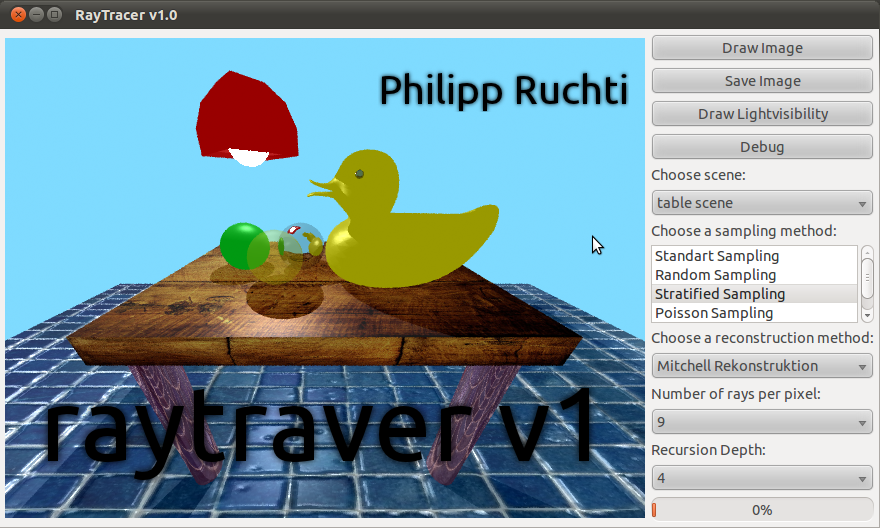
\includegraphics[width=\textwidth]{Bildschirmfoto.png}\\
	Ein Eindruck der GUI.\\
	\vspace{20pt}
	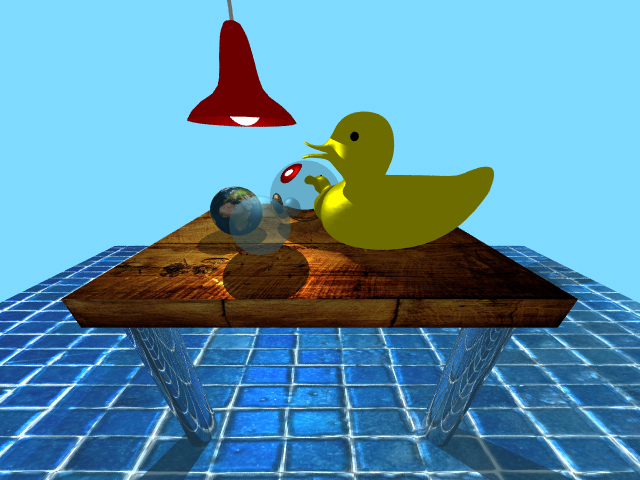
\includegraphics[width=\textwidth]{finish.png}\\
	Ein Beispielbild einer Szene mit Reflektionen und Transparenz.\\
\end{center}

\section*{Quellen}
\subsection*{C++Mathe-Bibliothek}
Für die hier verwendete Vektor- und Matrix-Mathematik wurde in dieser Implementierung die Mathebibliothek des Lehrstuhles für Mustererkennung und Bildverarbeitung von Prof. Brox verwendet. Copyright: Prof. Brox.

\subsection*{Weiterer Code}
Neben Qt und C++ wurde jeglicher weiterer Code persönlich angefertigt.
\end{document}